\documentclass[crop=false]{standalone}
\usepackage{graphicx}
\graphicspath{{images/}}
\usepackage{blindtext}
\usepackage{amsmath}

\begin{document}

\section{Lesson 3: The \textit{G(n,p)} model (ER Graphs) Erdős–Rényi}
This is the simplest random graph. It is not the same as the $G(N,L)$ graph, which has a fixed number of random links.
\subsection{Construction}
\begin{description}
    \item [n] Nodes
    \item [p] the probability any two nodes are connected 
\end{description}

\subsection{Properties}
Note how the LCC suddenly 'explodes' when the average node degree is greater than 1. This is called a phase transition. 
\begin{figure}
    \centering
    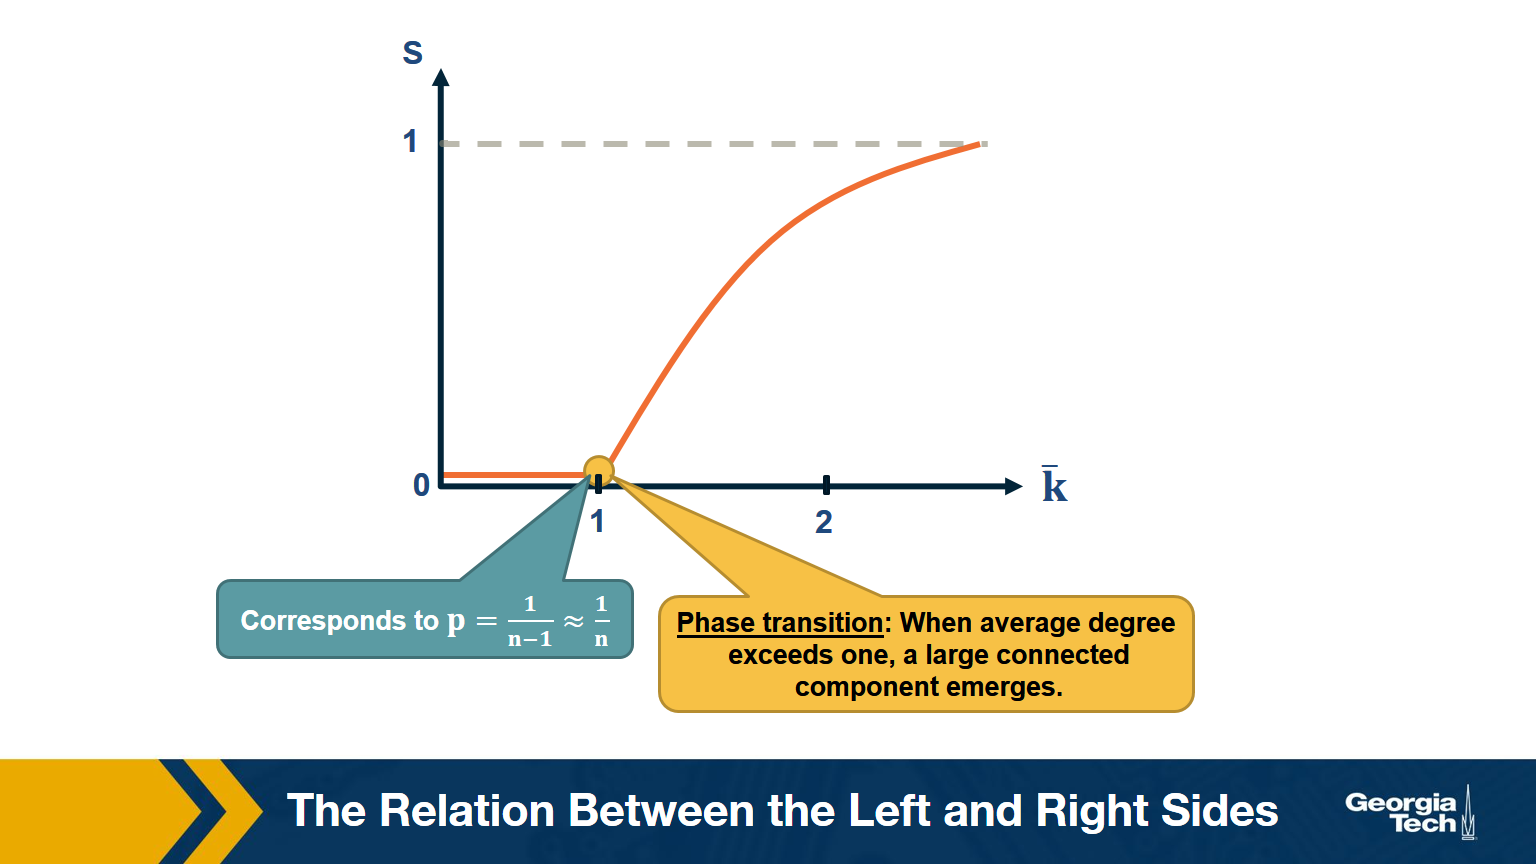
\includegraphics[width=1\linewidth]{lcc-explosion.png}
\end{figure}
\begin{description}
    \item [Degree Distribution]  $p_k\:=\:e^{-\overline{k}}\cdot{\frac{\overline{k}^{k}}{k!}},\:k=0,1,2,\dots$
    \item [average edges] $p\cdot{\binom{n}{2}}$
    \item [edges] expected number of edges is  $|E|=p\cdot\frac{n(n-1)}{2}$
    \item[LCC] Largest Connected Component
    \item[Degree = Link Count $P_L$]  $ P(Link Count = L) =( {\begin{array}{*{20}c} {\frac{{N(N - 1)}}{2}}  \\ L  \\ \end{array}} )p^L (1 - p)^{\frac{{N(N - 1)}}{2} - L}$
    \item [S] the probability that a node belongs to LCC\\
    $\overline{S} = S-1$ represents the probability that a node is \textbf{not} connected to a LCC
    $\overline{S}\:=\:((1-p)\:+\:p\cdot\overline{S})^{n-1}$\\
    $1-p$   Probability that a node is not connected to a randomly chosen other node.\\
    $p\cdot\overline{S}$ Probability that the node connects to a node \textbf{not in} the giant component.
    \item [average node degree] $p \cdot (n-1) $
    \item [average neighbor degree] at a $G(n,p)$ network is\\
    $\overline{k_{nn}}=\overline{k}\:+\:(1-p)$ using the Binomial distribution) or\\
    $\overline{k_{nn}}=\overline{k}\:+\:(1-p)$ using the Poisson approximation when $p\ll1$
\end{description}
\textbf{Question: how large should $p$ (or $k$) be so that the LCC covers all network nodes?}

Answer: The probability that a node does \textbf{not} connect to any node in the LCC $(1-p)^{S \, n}\approx(1-p)^n\:$if$\:S\approx1$

The expected number of nodes not connecting to LCC:
$\:n\cdot(1-p)^n\:=\:n(1-\frac{np}{n})^n\approx n\cdot e^{-n\cdotp}$

\end{document}
